\documentclass[a4paper,12pt]{article}

\usepackage{a4wide}
\usepackage{amsfonts}
\usepackage{amsmath}
\usepackage{amssymb}
\usepackage{lipsum}

\usepackage{graphicx}  % For including images

\usepackage{xcolor}  % For a colorfull presentation
\usepackage{listings}  % For presenting code 

\usepackage{hyperref}

% Definition of a style for code, matter of taste
\lstdefinestyle{mystyle}{
  language=Python,
  basicstyle=\ttfamily\footnotesize,
  backgroundcolor=\color[HTML]{F7F7F7},
  rulecolor=\color[HTML]{EEEEEE},
  identifierstyle=\color[HTML]{24292E},
  emphstyle=\color[HTML]{005CC5},
  keywordstyle=\color[HTML]{D73A49},
  commentstyle=\color[HTML]{6A737D},
  stringstyle=\color[HTML]{032F62},
  emph={@property,self,range,True,False},
  morekeywords={super,with,as,lambda},
  literate=%
    {+}{{{\color[HTML]{D73A49}+}}}1
    {-}{{{\color[HTML]{D73A49}-}}}1
    {*}{{{\color[HTML]{D73A49}*}}}1
    {/}{{{\color[HTML]{D73A49}/}}}1
    {=}{{{\color[HTML]{D73A49}=}}}1
    {/=}{{{\color[HTML]{D73A49}=}}}1,
  breakatwhitespace=false,
  breaklines=true,
  captionpos=b,
  keepspaces=true,
  numbers=none,
  showspaces=false,
  showstringspaces=false,
  showtabs=false,
  tabsize=4,
  frame=single,
}
\lstset{style=mystyle}

\begin{document}
\title{Machine Learning A (2023)\\Home Assignment 2}
\author{\color{red}Niels Moctezuma Krarup. Student ID: WTG176}
\date{}
\maketitle

% Please leave the table of contents as is, for the ease of navigation for TAs
\tableofcontents % Generates the table of contents
\newpage % Start a new page after the table of contents

\section{Illustration of Markov's, Chebyshev's, and Hoeffding's Inequalities (24 points)}

\subsection*{2a}
subsection 2a
\subsubsection*{1}
We start by plotting the empirical distribution based on 1e6 replications of observing the mean being above $\alpha \in \{0.5, 0.55,\dots , 0.95, 1\}$.

% Placeholder figure
\begin{figure}[htbp]
    \centering
    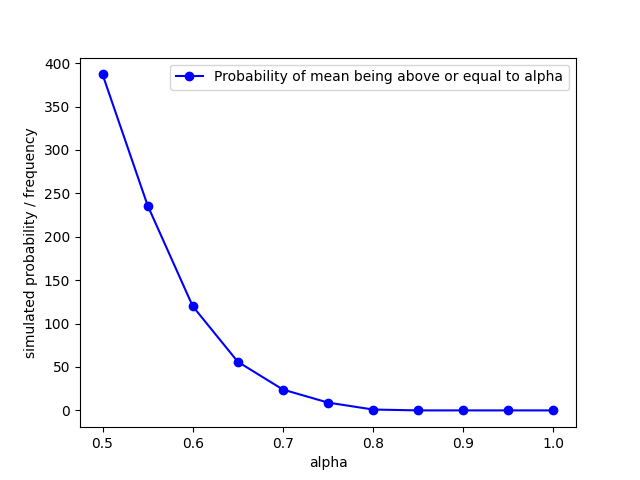
\includegraphics[width=0.5\linewidth]{HA2_2a_1.png}
    \caption{my captions} % Dummy caption generated using lipsum
    \label{fig:placeholder}
\end{figure}


\subsubsection*{2}
Since we take the mean of 20 Bernoulli random variables, the mean will only take on 21 different values, i.e. it will live on the space $\{0, \frac{1}{20},\dots , 1\}$. Due to having increments of size $\frac{1}{20}$ from adding another 'success' from one of the 20 realisations. Hence nothing new will be happening between the steps defined in the $\alpha$ vector. Of course if we were to increase $n$ this would change, as the mean would be more fine-grained.

\section{The Role of Independence (13 points)}
An easy but instrictive example is to make the $X_i$'s completely dependent of each other, that is $X_1 = X_n, n \geq 1$. \\
If we set $\mu = \mathbb{E} X_1 = 0.5$ then the mean will be either $0$ or $1$ for all $n \geq 1$ and the absolute difference to $\mu$ will hence be $\frac{1}{2}$ with probability $1$. 

Note that if we let $\mu \in (0,1)$ then the difference will only be greater than $\frac{1}{2}$ if the less likely outcome happens:
$$
\mathbb{P}\left( | \mu - \frac{1}{n}\sum_{i = 1}^n X_i  |   \geq \frac{1}{2} \right)  = \min(\mu, 1-\mu)
$$

\section{Tightness of Markov’s Inequality (Optional, question not for submission, 0 points)}

\section{The effect of scale (range) and normalization of random variables in Hoeffding's inequality (13 points)}

\section{Linear Regression (50 points)}

% Placeholder code
\begin{lstlisting}
# Example code
# Creating an example array
data = np.array([5, 2, 8, 1, 6])

# Calculating cumulative sum using cumsum
cumulative_sum = np.cumsum(data)
\end{lstlisting}

\bibliography{bibliography}  % If you have some references, use BibTeX

\end{document}